\section{Eigenvalue solution by Power Method on GPU}
The last problem concerns the evaluation of eigenvalue using the power method via a paralellized CUDA code. Reference for this implementation is a sequantial CPU-code provided by the course (\texttt{power\_cpu.cu}).\\

A scematic overview of the iteration loop for the power method is shown bellow in algorithm \autoref{alg:power_method}. 
\begin{algorithm}
    \caption{GPU Power Method}
    \label{alg:power_method}
    \begin{algorithmic}[1]
    \State \textbf{Input:} Matrix $\mathbf{A}$ of size $N \times N$, tolerance $\epsilon$, maximum iterations $max\_iter$
    \State \textbf{Output:} Dominant eigenvalue $\lambda$
    
    \State Initialize $\mathbf{v}$ with $v_1 = 1, v_i = 0$ for $i > 1$
    \State $\lambda_\text{Old} \gets 0$, $\lambda \gets 0$
    \State Allocate GPU memory for $\mathbf{A}$, $\mathbf{v}$, $\mathbf{w}$, and $\lambda$
    \State Copy $\mathbf{A}$ and $\mathbf{v}$ to GPU memory
    \State $\mathbf{w} \gets \mathbf{A} \cdot \mathbf{v}$ \Comment{First iteration of $\mathbf{w}$ computation using $\texttt{Av\_Product}$ kernel}
    
    \For{$i = 0$ to $max\_iter - 1$}
        \State Compute norm of $\mathbf{w}$: $\text{norm} \gets \sqrt{\mathbf{w}^T \cdot \mathbf{w}}$ \Comment{Using $\texttt{FindNormW}$ kernel}
        \State Normalize $\mathbf{v}$: $\mathbf{v} \gets \mathbf{w} / \text{norm}$ \Comment{Using $\texttt{NormalizeW}$ kernel}
        \State Compute $\mathbf{w} \gets \mathbf{A} \cdot \mathbf{v}$ \Comment{Using $\texttt{Av\_Product}$ kernel}
        \State Compute eigenvalue: $\lambda \gets \mathbf{v}^T \cdot \mathbf{w}$ \Comment{Using $\texttt{FindNormW}$ kernel}
        \If{$|\lambda - \lambda_\text{Old}| < \epsilon$}
            \State \textbf{Break} \Comment{Convergence achieved}
        \EndIf
        \State $\lambda_\text{Old} \gets \lambda$
    \EndFor
    
    \State Copy $\lambda$ back to host memory
    \State Deallocate GPU memory
    \end{algorithmic}
\end{algorithm}

\textbf{Note:} A $sqrt()$ was added in the \texttt{NormalizeW} kernel over \texttt{g\_NormW[0]}. This way we can use the output of \texttt{FindNormW} directly in the \texttt{NormalizeW} kernel.\\

All of the following benchmarks are perfromed in the supplied IPython notebook on Google Collab using T4 GPUs. 

\subsection{Step 1: Shared vs. global memory for matrix-vector multiplication}
To investigate the performance impact of shared vs. global memory during the matrix vector multiplication we first need an alternative kernel which doesn't use shared memory. This kernel is given bellow: 
\lstinputlisting[language=c]{input/code/03/Av_Product_Global.c}
Subsequently, 10 measurements are perfromed with the original kernel and the changed kernel to determine the mean times depending on memory usage patterns. 
We obtain a \Shining{scatter plot} seen in \autoref{fig:cuda_step1}
\begin{figure}[H]
    \centering
    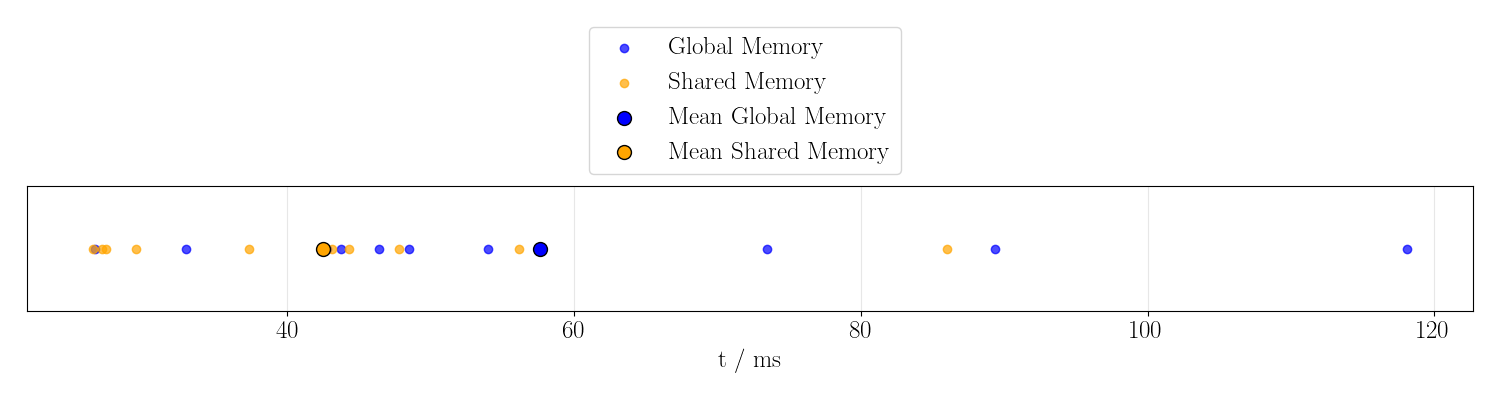
\includegraphics[width=\textwidth]{../fig/lab3/step1.png}
    \caption{Measurements }
    \label{fig:cuda_step1}
\end{figure}
Furthermore, we obtain a mean time using global memory of $t_{global} = \SI{576(7)}{\milli\second}$ and by using shared memory in this kernel we get $t_{shared} = \SI{425(3)}{\milli\second}$. 
This means we have time savings of $\SI{26(1)}{\percent}$ or about $\nicefrac{1}{4}$ when using shared memory compared to global memory. 
\subsection{Step 2: Execution time for different N and threads per block}
I implemented a small loop to run the GPU code for 5 different $N$ with $N \in \{50, 500, 2000, 4000, 5000\}$. The resulting time benchmarks for 32, 64 and 100 threds per block can be seen in \autoref{fig:cuda_step2}. 
\begin{figure}[H]
    \centering
    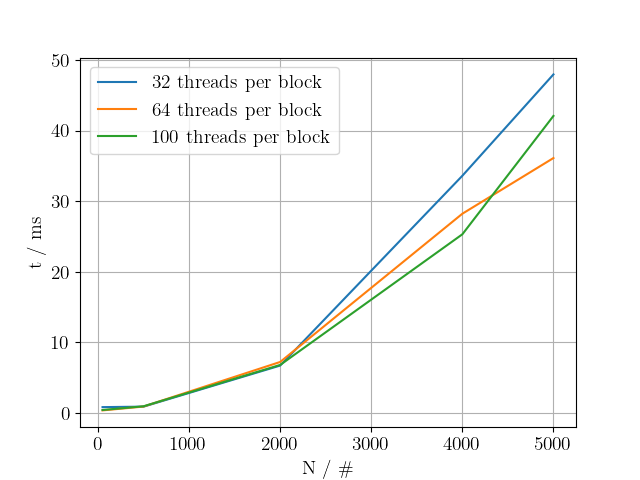
\includegraphics[width=0.5\textwidth]{../fig/lab3/step2.png}
    \caption{Runtime for $N \in \{50, 500, 2000, 4000, 5000\}$ and for 32, 64 and 100 threads per block respectively.}
    \label{fig:cuda_step2}
\end{figure}
\TODO{maybe add somethin, justification whatever?!}
\subsection{Step 3: Speedups}
We measure two different scenarios: 
\begin{enumerate}[i]
    \item excluding time of memory copy from CPU $\rightarrow$ GPU
    \item including time of memory copy from CPU $\rightarrow$ GPU
\end{enumerate}
After measuring \Shining{5} rounds without (i) and with (ii) memory access time we obtain the following \Shining{scatter plot} in \autoref{fig:cuda_step3}
\begin{figure}[H]
    \centering
    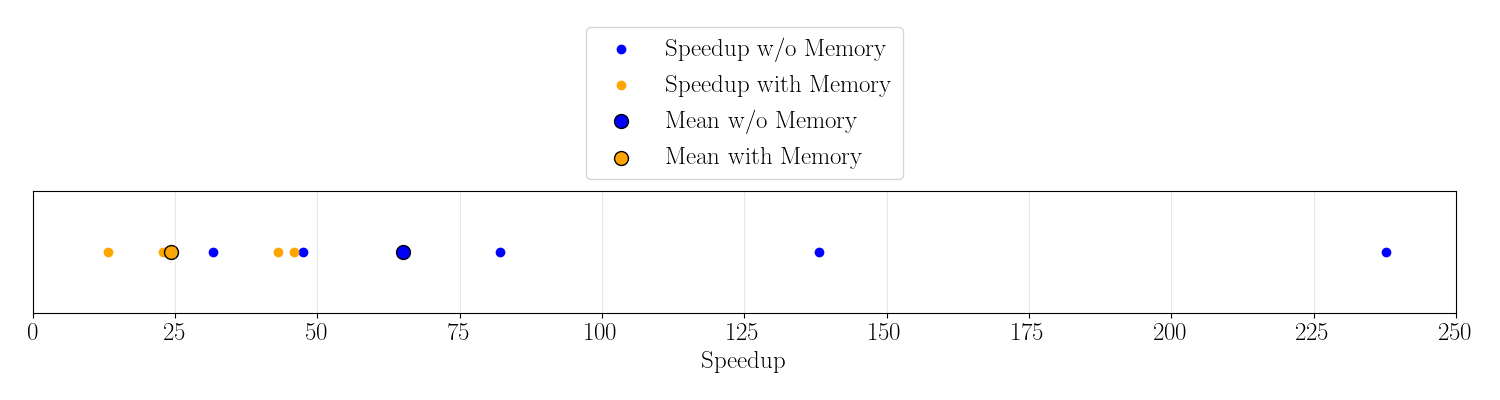
\includegraphics[width=\textwidth]{../fig/lab3/step3.png}
    \caption{Speedup of GPU implementation vs. CPU with and without memory transfer times.}
    \label{fig:cuda_step3}
\end{figure}
The mean speedup without memory access times is $\times 65$ and with memory access timed it comes out to $\times 24$.
\subsection{Step 4: Explanation of the results}
